\documentclass[UTF8]{ctexart}
\usepackage[]{ctex}
\usepackage{natbib}
\usepackage{graphicx}
\usepackage{enumitem}
\usepackage{setspace}
\usepackage{float}
\bibliographystyle{plain}

\title{Cuckoo 性能测试报告}
\author{杨景凯 520021910550}
\date{2022年 5月 14日}

\begin{document}

\begin{center}
    \quad \\
    \quad \\
    \kaishu \fontsize{45}{17} 上\quad 海\quad 交\quad 通\quad 大\quad 学
    \vskip 3.5cm
    \heiti \zihao{2} Cuckoo 性能测试\\
    实验报告
\end{center}
\vskip 3.5cm
\begin{quotation}
    \songti \fontsize{30}{30}
    \doublespacing
    \par\setlength\parindent{12em}
    \quad 
\begin{center}
    学\hspace{0.61cm} 院:\underline{电子信息与电气工程学院}

    学生姓名:\underline{\qquad    \quad \quad 杨景凯    \quad  \quad\qquad }

    学\hspace{0.61cm} 号:\underline{\quad \quad\quad520021910550\quad\quad}
\end{center}
    \centering
    2022年5月14日
\end{quotation}

\clearpage
\tableofcontents

\clearpage
\section{背景介绍\cite{refpdf1}}
\subsection{哈希表}
哈希表是一种可以快速寻找目标键值对的方式,但是在多个键对应的哈希值相同时就会
发生“冲突”。为了应对这种冲突,不同的哈希表会有不同的冲突应对策略——线性哈希在对
应哈希值的基础上继续向下查找空位,并将其放在第一个空位上;链式哈希表则会将对应哈
希值的所有键值对串成链表,查找时遍历链表。
\subsection{Cuckoo 哈希}
Cuckoo 采用了不同的设计来减少冲突情况下查找的代价。即每个键有且只有两个不同
的哈希值,如果两个哈希值对应的位置存在空位就存放在其中。如果两个哈希值对应的位置
不存在空位,那就需要转移对应位置中已有的键值对,直到所有键值对都落在它们两个哈希
值之一对应的指定位置处。
当然这种方法在键值对转移过程中可能会出现死循环,解决方法是路径检测加上重新哈
希。检测循环路径的方法也比较简单,可以预先设定一个阈值,当循环次数或者递归调用次
数超过设定阈值时,就可以认为产生了循环路径。

\section{测试}
\subsection{测试内容}
以哈希表容量为 100000 为例,在负载因子为 0.1, 0.5, 0.75, 1.0 的情况下,插入数据并测试 Cuckoo 哈希的查找时间(测试查找成功的情况即可)

\subsection{测试方式}
测试方式如下:

1. 先将总数据量为$100000 \cdot \alpha$($\alpha$表示负载因子)的数据顺序插入Cuckoo 哈希表中,对于插入数据,我选取了简单的$0 \sim 100000 \cdot \alpha$的数据。

2. 将所有数据(即$0 \sim 100000 \cdot \alpha$的数据,共计$100000 \cdot \alpha$个)进行搜索,每一数据搜索1000次,并除以$1000 \cdot \alpha$,计算得到搜索任意一个数据的平均查找时间乘以100000的时间(ms)。

\subsection{测试结果}
测试结果如下表与图所示:

\begin{table}[H]
    \centering
    \begin{tabular}{|c|c|c|c|c|}
        \hline
        负载因子&	0.1&	0.5&	0.75&	1\\
        \hline
        乘以100000后的平均查找时间(ms)&	0.45&	0.42&	0.425333333&	0.424\\
        \hline
    \end{tabular}
    \caption{Cuckoo哈希表容量为100000时负载因子与平均查找时间(ms)关系表格}
\end{table}

\begin{figure}[H]
    \centering
    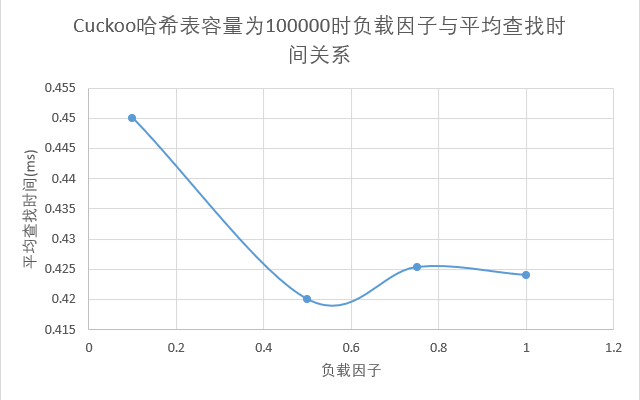
\includegraphics[scale=0.7]{T-alpha.png}
    \caption{Cuckoo哈希表容量为100000时负载因子与平均查找时间(ms)关系图}
\end{figure}

\section{结论}
观察表格与图片可以发现,Cuckoo哈希表容量为100000时,负载因子与平均查找时间没有关系,不同负载因子下,对于Cuckoo哈希表的平均查找时间相近,故可以证明Cuckoo哈希表是一种优秀的查找数据的结构。

\clearpage
\begin{thebibliography}{99}
    \bibitem{refpdf1}Cuckoo 性能测试.pdf
\end{thebibliography}
\end{document}
